\documentclass[10pt,twoside]{article}
\usepackage[utf8]{inputenc}
\usepackage{amsmath}
\usepackage{amsfonts}
\usepackage{amssymb}
\usepackage[spanish,es-noshorthands]{babel}
\usepackage[T1]{fontenc}
\usepackage{lmodern}
\usepackage{graphicx,hyperref}
\usepackage{tikz,pgf}
\usepackage{multicol}
\usepackage{subfig}
\usepackage[papersize={6.5in,8.5in},width=5.5in,height=7in]{geometry}
\usepackage{fancyhdr}
\pagestyle{fancy}
\fancyhead[LE]{
\includegraphics[height=12pt]{Images/logo-colegio.png} Cálculo $11^{\circ}$}
\fancyhead[RE]{}
\fancyhead[RO]{\textit{Germ\'an Avenda\~no Ram\'irez, Lic. U.D., M.Sc. U.N.}}
\fancyhead[LO]{}

\author{Germ\'an Avenda\~no Ram\'irez, Lic. U.D., M.Sc. U.N.}
\title{\begin{minipage}{.2\textwidth}

\includegraphics[height=1.75cm]{Images/logo-colegio.png}\end{minipage}
\begin{minipage}{.55\textwidth}
\begin{center}
Taller, Calculando límites con tablas y gráficas \\
Cálculo $11^{\circ}$
\end{center}
\end{minipage}\hfill
\begin{minipage}{.2\textwidth}

\includegraphics[height=1.75cm]{Images/logo-sed.png} 
\end{minipage}}
\date{}
\begin{document}
\maketitle
Nombre: \hrulefill Curso: \underline{\hspace*{44pt}} Fecha: \underline{\hspace*{2.5cm}}

1--6 Complete la tabla de valores hasta 5 lugares decimales y use ésta para estimar el valor del límite
\begin{enumerate}
 \item $\displaystyle{\lim_{x\rightarrow4}\dfrac{\sqrt{x}-2}{x-4}}=$ \hfill
\begin{tabular}{|l|l|l|l||l|l|l|}\hline
$x$ & 3.9 & 3.99 & 3.999 & 4.001 & 4.01 & 4.1\\\hline
$f(x)$ &  &  &  &  &  & \\\hline
                                                           \end{tabular}                                                                                                                      
\item $\displaystyle{\lim_{x\rightarrow2}\dfrac{x-2}{x^{2}+x-6}}=$\hfill
\begin{tabular}{|l|l|l|l||l|l|l|}\hline
$x$ & 1.9 & 1.99 & 1.999 & 2.001 & 2.01 & 2.1\\\hline
$f(x)$ &  &  &  &  &  & \\\hline
\end{tabular}
\item $\displaystyle{\lim_{x\rightarrow1}\dfrac{x-1}{x^{3}-1}}$ \hfill
\begin{tabular}{|l|l|l|l||l|l|l|}\hline
$x$ & 0.9 & 0.99 & 0.999 & 1.001 & 1.01 & 1.1\\\hline
$f(x)$ &  &  &  &  &  & \\\hline
\end{tabular}
\item $\displaystyle{\lim_{x\rightarrow0}\dfrac{e^{x}-1}{x}}=$ \hfill
\begin{tabular}{|l|l|l|l||l|l|l|}\hline
$x$ & --0.1 & --0.01 & --0.001 & 0.001 & 0.01 & 0.1\\\hline
$f(x)$ &  &  &  &  &  & \\\hline
\end{tabular}
\item $\displaystyle{\lim_{x\rightarrow0}\dfrac{\sin(x)}{x}}=$\hfill
\begin{tabular}{|l|l|l|l|l|l|}\hline
$x$ & $\pm1$ & $\pm0.5$ & $\pm0.1$ & $\pm0.05$ & $\pm0.01$ \\\hline
$f(x)$ &  &  &  &  & \\\hline
\end{tabular}
\item $\displaystyle{\lim_{x\rightarrow 0^{+}}x\ln(x)}=$ \hfill
\begin{tabular}{|l|l|l|l|l|l|}\hline
$x$ & 0.1 & 0.01 & 0.001 & 0.0001 & 0.00001\\\hline
$f(x)$ &  &  &  &  & \\\hline
\end{tabular}

7--12 Use la tabla de valores para estimar el valor del límite. Luego use ``geogebra'' para graficar la función y confirmar sus resultados.
\begin{multicols}{2}
\item $\displaystyle{\lim_{x\rightarrow -4}\dfrac{x+4}{x^{2}+7x+12}}=$
\item $\displaystyle{\lim_{x\rightarrow 1}\dfrac{x^{3}-1}{x^{2}-1}}=$
\item $\displaystyle{\lim_{x\rightarrow 0}\dfrac{5^{x}-3^{x}}{x}}=$
\item $\displaystyle{\lim_{x\rightarrow 0}\dfrac{\sqrt{x+9}-3}{x}}=$
\item $\displaystyle{\lim_{x\rightarrow 1}\left(\dfrac{1}{\ln(x)}-\dfrac{1}{x-1}\right)}=$
\item $\displaystyle{\lim_{x\rightarrow 0}\dfrac{\tan(2x)}{\tan(3x)}}=$
\end{multicols}
\item Para la función $f$ cuya gráfica se dá, determine el valor pedido si existe. Si no existe, explique por qué

\begin{minipage}{.6\textwidth}
\begin{enumerate}
\begin{multicols}{2}
 \item $\displaystyle{\lim_{x\rightarrow 1^{-}}f(x)}=$
 \item $\displaystyle{\lim_{x\rightarrow 1^{+}}f(x)}=$
 \item $\displaystyle{\lim_{x\rightarrow 1}f(x)}=$
 \item $\displaystyle{\lim_{x\rightarrow 5}f(x)}=$
 \item $f(5)=$
 \item $f(-1)=$
 \end{multicols}
 \end{enumerate}
\end{minipage}
\begin{minipage}{.35\textwidth}
 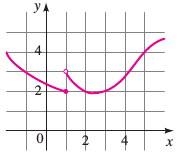
\includegraphics[scale=.75]{./Images/funcionPto13.png}
% funcionPto13.png: 0x0 pixel, 300dpi, 0.00x0.00 cm, bb=
\end{minipage}
\item Para la función $f$ cuya gráfica se da, determine el valor pedido si existe. Si no existe, explique por qué.
 \begin{minipage}{.6\textwidth}
 \begin{enumerate}
 \begin{multicols}{2}
  \item $\displaystyle{\lim_{x\rightarrow 0}f(x)}=$
  \item $\displaystyle{\lim_{x\rightarrow 3^{-}}f(x)}=$
  \item $\displaystyle{\lim_{x\rightarrow 3^{+}}f(x)}=$
  \item $\displaystyle{\lim_{x\rightarrow 3}f(x)}=$
  \item $f(3)=$
  \item $f(0)=$
  \end{multicols}
  \end{enumerate}
  \end{minipage}
  \begin{minipage}{.35\textwidth}
 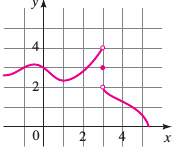
\includegraphics[scale=.75]{./Images/funcionPto14.png}
% funcionPto14.png: 0x0 pixel, 300dpi, 0.00x0.00 cm, bb=
\end{minipage}




\end{enumerate}

\end{document}
